\documentclass[a4paper,dvipsnames]{article}

\input ../header
\newcommand{\checkedbox}{\makebox[0pt][l]{$\square$}\raisebox{.15ex}{\hspace{0.1em}$\checkmark$}}
\newcommand{\checkbox}{\makebox[0pt][l]{$\square$}\raisebox{.15ex}{\hspace{0.1em}}\hspace{3mm}}

\begin{document}

\title{Évaluation 4 -- Sujet B -- Éléments de correction}
\author{}
\date{}

\maketitle{}

\pagestyle{empty}

\exo\vspace{-2mm} 
\begin{enumerate}
  \item Écrire chaque nombre sous la forme $a\sqrt{b}$, où $a$ est un entier et $b$ l'entier naturel le plus petit possible.

    \begin{enumerate}
      \item $\color{red}\sqrt{125}=\underbrace{\sqrt{25}}_{=5}\times\sqrt{5}=5\sqrt{5}$.
      \item $\color{red}\sqrt{30}\times\sqrt{20}=\sqrt{600}=\sqrt{100}\times\sqrt{6}=10\sqrt{6}$
      \item $\color{red}3\sqrt{5}-\sqrt{20}+3\sqrt{45}=3\sqrt{5}-\sqrt{4}\times\sqrt{5}+3\times\sqrt{9}\times\sqrt{5}=3\sqrt{5}-2\sqrt{5}+9\sqrt{5}=10\sqrt{5}$
    \end{enumerate}
  \item Écrire sans racine carrée au dénominateur :

    \begin{multicols}{2}
      \begin{enumerate}
	\item $\color{red}\dfrac{3}{\sqrt{11}}=\dfrac{3\sqrt{11}}{\sqrt{11}\times\sqrt{11}}=\dfrac{3\sqrt{11}}{11}$
	\item $\color{red}\dfrac{3}{\sqrt{6}+1}=\dfrac{3(\sqrt{6}-1)}{(\sqrt{6}+1)(\sqrt{6}-1)}=\dfrac{3(\sqrt{6}-1)}{5}$
      \end{enumerate} 
    \end{multicols}

  \item Donner une valeur arrondie de $\dfrac{3}{\sqrt{11}}$ à $10^{-4}$ près, puis un encadrement d'amplitude $10^{-3}$ de $\dfrac{3}{\sqrt{6}+1}$.\\
    On obtient, grâce à la calculatrice, $\color{red}\dfrac{3}{\sqrt{11}}\approx \np{0,9045}$ et $\color{red}\np{0,869}\leq \dfrac{3}{\sqrt{6}+1}\leq \np{0,870}$.
\end{enumerate}

\bigskip

\exo On fait tourner chacune des roulettes suivantes et on note la couleur obtenue. Modéliser chaque expérience aléatoire en complétant le tableau donné.

\begin{multicols}{2}
  \begin{center}
    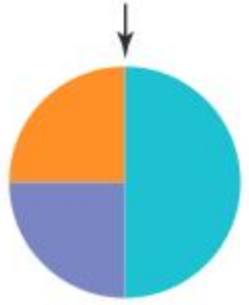
\includegraphics[width=2.5cm]{evaluation_4_figure_2.png}
  \end{center}

  \begin{center}
    \vspace*{0.7cm}
    \hspace*{-3cm}\begin{tabular}{@{}cccc@{}}
      \toprule
      Couleur obtenue & vert & orange & bleu\\
      \midrule
      Probabilité & $\color{red}\dfrac{1}{2}$ & $\color{red}\dfrac{1}{4}$ & $\color{red}\dfrac{1}{4}$\\
      \bottomrule
    \end{tabular}
  \end{center}
\end{multicols}

\begin{multicols}{2}
  \begin{center}
    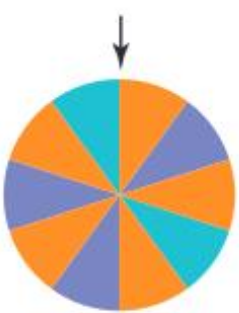
\includegraphics[width=2.3cm]{evaluation_4_figure_3.png}
  \end{center}

  \begin{center}
    \vspace*{0.75cm}
    \hspace*{-3cm}\begin{tabular}{@{}cccc@{}}
      \toprule
      Couleur obtenue & vert & orange & bleu\\
      \midrule
      Probabilité & $\color{red}\dfrac{2}{10}$ & $\color{red}\dfrac{5}{10}$ & $\color{red}\dfrac{3}{10}$\\
      \bottomrule
    \end{tabular}
  \end{center}
\end{multicols}

\bigskip

\exo On considère la fonction (incomplète) suivante écrite en Python :

\begin{minted}{python}
def inconnue(b, h):
    a = ...
    return ...
\end{minted}

\begin{enumerate}
  \item Comment s'appelle cette fonction ?\\
    {\color{red}Cette fonction s'appelle \mintinline{python}{inconnue}.}
  \item Combien de paramètres possède-t-elle ?\\
    {\color{red}Elle possède 2 paramètres.}
  \item Quel mot-clé permet de préciser ce que renvoie une fonction en Python ?\\
    {\color{red}Il s'agit du mot-clé \mintinline{python}{return}.}
  \item Compléter la fonction afin qu'elle renvoie l'aire d'un triangle de base $b$ et de hauteur $h$.\\
    \textit{Remarque. -- On rappelle que l'aire d'un tel triangle est donnée par la formule :
      \[\dfrac{b\times h}{2}.\]
  }
\begin{minted}{python}
def inconnue(b, h):
    a = b * h / 2
    return a
\end{minted}
\item Comment utiliser cette fonction afin de déterminer l'aire d'un triangle de base $10$ et de hauteur $7$ ?\\
  {\color{red}Il suffit d'écrire \mintinline{python}{inconnue(10, 7)}.}
\end{enumerate}

\end{document}
